\chapter{Maze complexity problems}\label{cha:background}
One of the main puropse of this paper is to discuss a complexity of a maze. In this chapter I would like to review all existing methods of determining the complexity of a maze problem.
It is important to precisly define what complexity means and the implication of such definition. The simplest meaning of the question: \textit{is this maze complicated}, is how dificult it is to find a way out? Or, How difficult it is to move from point A to point B in this maze?
But there could be also another approach: \textit{how difficult it is to generate such maze}, meaning how rare is a particular maze. Below I will try to collect all major definition of maze and graphs complexity, and discuss why it's important to know the complexity of a maze problem. 
And what are the tools to study this complexity. Further in chapter 5 I will also provide a deeper analisis. {coś tu dopisać jeszcze bo nie brzmi to dobrze }
\section{Complexity measures in Graph Theory}
In below part I will present the approaches derived from graph theory which allows to describe and measure complexity of a graph. 
Conventionally graph complexity in graph theory is defined by measures such as degree distribution, clustering coefficient, edge density, community.Another approach which derived from classical information theory is to 
generate graphs with some paricularieties while being random in all other respects and then compare and decide is this particular characteristic is typical among group of graphs. There is also a recent advanced idea to use a \textit{principle of maximum entropy} or Maxent to estimate the algoritmic complexity of a graph. The main idea 
of maximum entropy concept is that the more statistical random graph is the more typical. \cite{HeZeni}
\begin{definition}\textbf{A Degree Distribution}  $P(k) = \frac{n_k}{n}$ is defined as a proportion of vertex with a degree $k$ to all vertices in a graph. \end{definition}  
\begin{definition}\textbf{A Clustering Coeficient} $C_i$ is defined as a proportion of vertex links to vertex possible links. The coefficient for an undirected graph might be given by $C_i = \frac{k_i(k_i-1)}{2}$ where $k_i$ are the neighbours of vertex $v_i$. The average clustering coefficient is given by $\bar{C} = \frac{1}{n}\sum_{n = 1}^{n} C_i $\end{definition}
\begin{definition}\textbf{A Community} is a subset of vertices denseley connected respectively, and loosely connected to vertices in other communieties in the same graph.\end{definition}
\begin{definition}\textbf{A Graph Entropy} "Graph entropy measures represent information-theoretic measures for characterizing networks quantitatively"\cite{MaDehm}. It is the most important and difficult measure to determine graph complexity. There is no "good enough" definition of graph entropy which could be applied to all different kind of problems. Searching new ways of calculating the entorpy of the graph systems is a huge challange for scientist from mathematics, physics, bilogy, chemistry, coputer and sociology sciences. We can didistinguish 3 major fields of graph entropy: The Classical Entropy, The Deterministic Entropy and The Propabilistic Entriopyt. All three have different application, sometimes very specific.  As a result, I will not try to make here a general definition of graph entropy, but instead in the next subsection I will provide some more details abous Shannon's entropy measure which is one of the simplest method and will  be used later in this paper to calulate maze complexity. 
\end{definition}  
\subsection{Shannon Entropy}
Shanon entropy derives directly from Boltzmann entropy in thermodynamics. "Shannon’s concept of information entropy quantifies the average number of bits needed to store or communicate a message."\cite{HeZeni}. In a sense of complexity, the Shanonn entropy measures, how complex the string of a graph problem must be to avoid loosing any information about it's state. The main concept is that the information buid by $n$ different symbols, can not be stored in lest than $log(n)$ bits.
Shanon entropy of the object $M(R, p(x_i))$ is given by ()\cite{HeZeni}:
\begin{equation}
H(M) = - \sum_{n = 1}^{n} p(x_i)\log_2 p(x_i)
\end{equation}
\textbf{Where:}\\
$R$ is set of possible outcomes, eh. All posiible adjacency matrix of size $m$\\
$p(x_i)$ is a propability of outcome $R$,\\
$n= |R|$\\
\section{Complexity measures in Mazes}
In this section I will discuss the characteristics which influences the complexity of a maze. I will try to make an overview of different approaches and will try to compare them. 
One of the main aim of this work is a analysis and research to define and describe different measures of maze complexity problem. 
\subsection{Independant Maze Parameters}
\begin{description}[style=unboxed]
    \item[Size] One of the most evident complexity factors is size of a maze. In this work we use a definition of a maze which is reprezented as a square grid which size is denoted by $s_m = nxm$. It's almost to easy to think that small maze is a simple maze, and huge maze is a diffcult one.
    \begin{figure}[!h]
        \centering
        \begin{subfigure}{.5\textwidth}
          \centering
          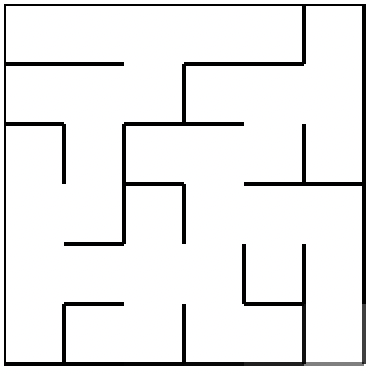
\includegraphics[width=.5\linewidth]{66}
          \caption{An Aldous-Broder maze with $s_m = 6x6$}
          \label{fig:sub1}
        \end{subfigure}%
        \begin{subfigure}{.5\textwidth}
          \centering
          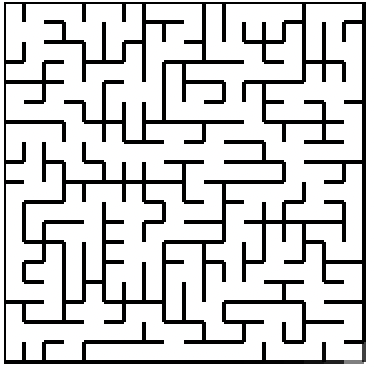
\includegraphics[width=.5\linewidth]{1818}
          \caption{An Aldous-Broder maze with $s_m = 18x18$}
          \label{fig:sub2}
        \end{subfigure}
        \caption{Examples of different size mazes}
        \label{fig:test}
        \end{figure}
        \item[Path lenght] Another key characteristic determinng the complexity of a maze is the average lenght $\bar{p_l}$ of the paths. The longer the path, the bigger the risk of following faulty road to solution. A Path in this case is considered as a sequence of moves from the start to each dead-end in acyclic mazes.In cyclic mazes paths can be infinite. 
        \begin{figure}[!h]
            \centering
            \begin{subfigure}{.5\textwidth}
              \centering
              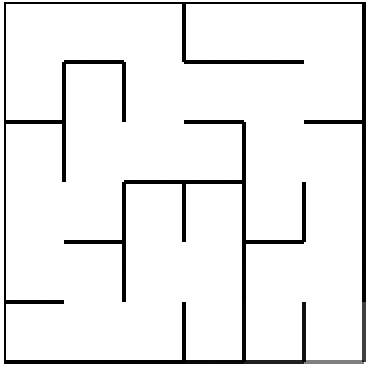
\includegraphics[width=.5\linewidth]{aldous}
              \caption{An Aldous-Broder maze with $\bar{p}_l = 9.42$}
              \label{fig:sub1}
            \end{subfigure}%
            \begin{subfigure}{.5\textwidth}
              \centering
              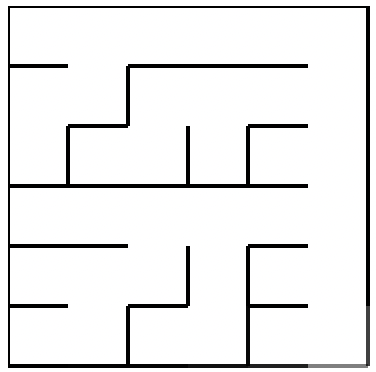
\includegraphics[width=.5\linewidth]{binary}
              \caption{A Binary Tree maze with $\bar{p}_l = 10.8$}
              \label{fig:sub2}
            \end{subfigure}
            \caption{Examples of different average path lenght mazes}
            \label{fig:test}
            \end{figure}
        \item[Density] Density for an acyclic graph is given by (\ref{acyclic_density}), and density for cyclic maze is given by (\ref{cyclic_density})\cite{SBorg}. It describes the ratio between number of all possible connection and the existing number of connections ( edges) 
        \begin{figure}
            \centering
            \begin{subfigure}{.5\textwidth}
              \centering
              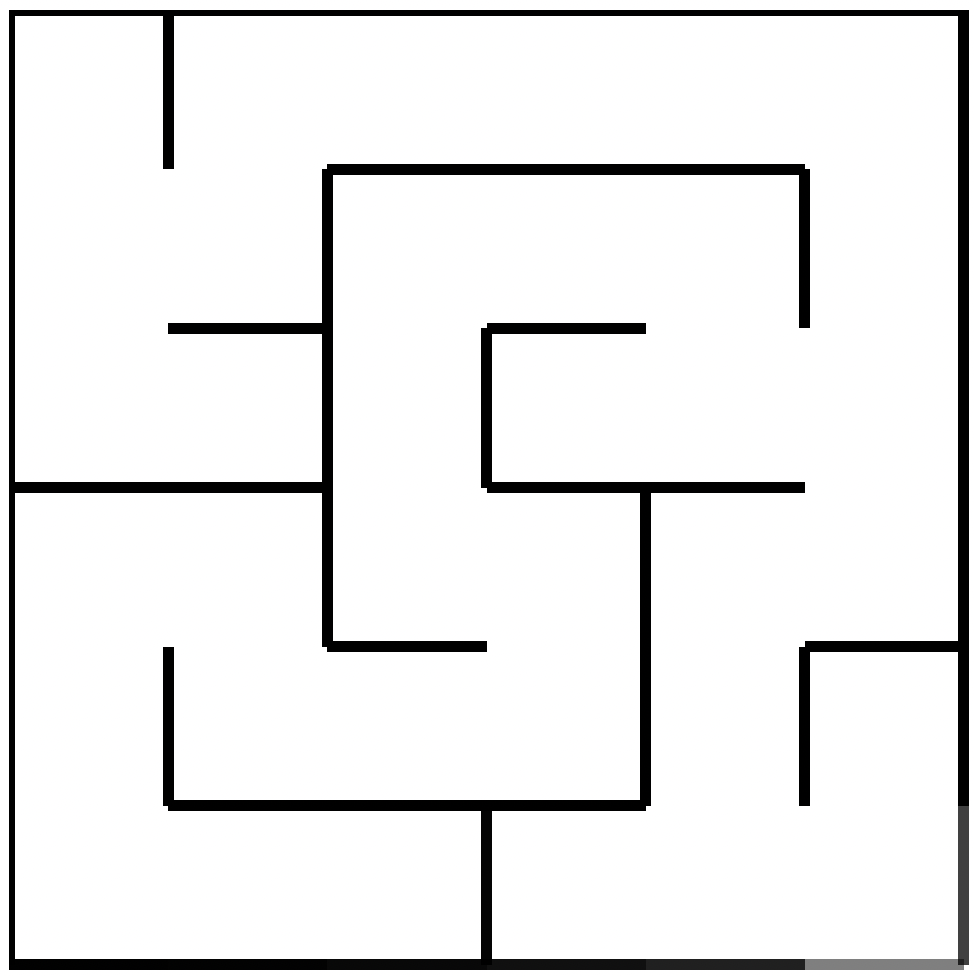
\includegraphics[width=.5\linewidth]{recursivedens}
              \caption{A Recoursive-Backtracker maze with $density = 0.40$}
              \label{fig:sub1}
            \end{subfigure}%
            \begin{subfigure}{.5\textwidth}
              \centering
              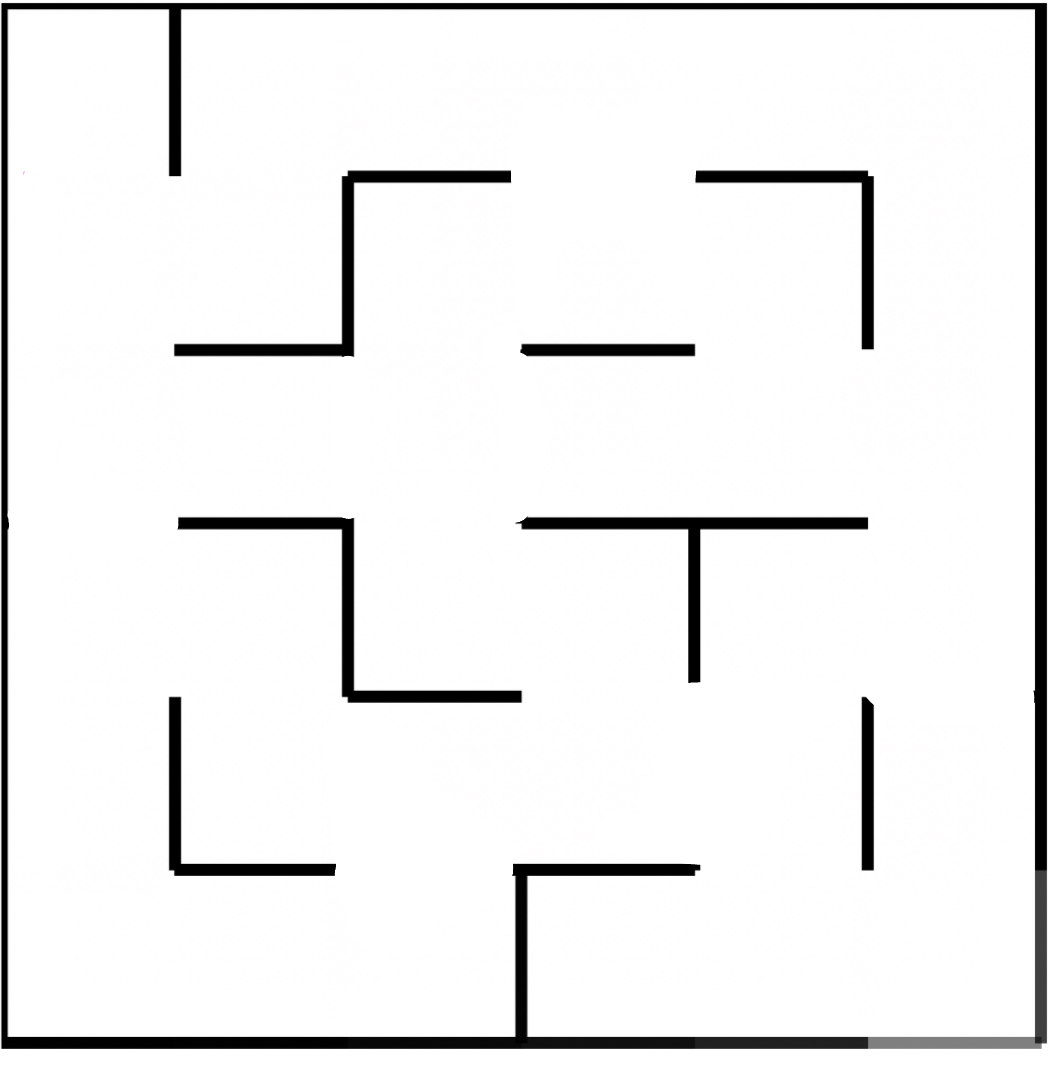
\includegraphics[width=.5\linewidth]{recursivedensecyclic}
              \caption{A Binary Tree maze with $density = 0.50$}
              \label{fig:sub2}
            \end{subfigure}
            \caption{Examples of different density mazes}
            \label{fig:test}
            \end{figure}
\end{description}

\subsection{McClendon Measure}
There are not many sources indicating a quantitative study of the measure of maze complexity. One of the most cited work in this field is a McClendon study of maze diffuculty and complexity.
McClendon's work treats about maze complexity and difficulty in continous measure using continuum theory.
Main presupositions of the work are that the maze is a perfect maze type, there are two distinguished pair of points $(p,q)$ in the maze $M$ called gates. Where $p$ is an entrance and $q$ is an exit. A maze is build by hallways $h$. Where hallways are a subsets $K$ of $M$ with the $degree = 2$. A subset $W_h = {w_1,w_2,\cdots, w_n}$ of $h$ incorporates all points of $h$.
A trail is a path in the maze build by hallways. The branch is any trail intersecting the solution $T$ of a maze. Each branch in $M$ is connected to $T$ by a point $v_i$ in $I$ which is a intersections set $I = {v_1,v_2,\dots, v_n}$.
The McClendon's complexity of a hallway $h$ is given by:\\
\begin{equation}
\gamma(h) = D(h)\sum_{n = 1}^{n} \frac{\theta(w_i)}{d(w_i)\cdot \pi}
\end{equation}
\textbf{Where:}\\
 $D(h)$ is an arclength of $h$,\\
 $\theta(w_i)$ is the absolute value of the difference in the radian measures between the directions $V(t_i)$ and $V(t_{t+1})$\\
 $d(w_i)$ is a lenght of a arc between $w_{i-1}$ and $w_i$ in $W_h$.\\
 \newline
The McClendon's complexity of a Maze $M$ is given by:\\
\begin{equation}
\gamma(M)=\log\bigl[\gamma(T) + \sum_{n = 1}^{n} \gamma(B_i)  \bigr] 
\end{equation}
\textbf{Where:}\\
$\gamma(T)$ is a complexity of a solution of the maze\\,
$\gamma(B_i) = \sum_{n = 1}^{n} \gamma(h_i)$ is a complexity of a branch $B_i$.\\
\newline In the method above to calculate the complexity of a maze we must know the solution of the maze. To avoid this we should use the extrinsic approximation of the above method which is given by:\\
\begin{equation}
\gamma(M) \approx \log \bigl[\sum_{n =1}^{n}\gamma(h_i)\bigr]
\end{equation}
\textbf{Where:}\\
$y(h_i)$ is the complexity of $h_i$\\ 
\newline
In this paper we are using the square grid to generate and solve mazes. As a result of uniform grid, the McClendon measure will be simplified, and caluclated as:
\begin{equation}
 \gamma(M) \approx \log  \bigl[\sum_{n =1}^{n}\frac{h(i)_l\cdot \mathcal{T}}{2}\bigr]
\end{equation}
\textbf{Where:}\\
$h(i)_l$ is the total length of the hallway,\\
$\mathcal{T}$ is the total number of L turns in the hallway, and each L turn is 90$^\circ$.

%porownac to co wyjdzie z tym wykresem w tej pracy 

\subsection{Time Complexity of maze generators}

  \begin{table}[!h]
    \begin{center}
  \begin{tabular}{ |p{6cm}||p{3cm}|  }
    \hline
    Maze Generator Algorithm  Name& Time Complexity\\
    \hline
    Binary Tree  & $O(|V|)$\\
    Aldous-Broder& $O(|V|^3)$ \\
    Recursive- Backtracker& $O(|V|+|E|)$\\
    \hline
   \end{tabular}
   \caption{\label{tab:table-name}Your caption.}
  \end{center}
  \end{table}

\subsection{Distinctivness and uniquness of a maze}

%typical path lenght
%człowiek a komputer
%how many visited cells during solution
%zgodny z heurystyką